% =====================================================================
%  Chapter 23 — The Thermal and Power Budget
% =====================================================================

\chapter{The Thermal and Power Budget}
\label{ch:thermal-budget}

The mid-infrared channel is where the lunar proposal is weakest, and the
arithmetic is unusually clean. This chapter works through it, because a
reader is entitled to know where the argument loses, and because the place
it loses is a place where a better platform already exists.

\section{The ground is brighter than the target}

Sunlit lunar regolith reaches about 390 kelvin. By Wien's displacement law,
a blackbody at that temperature radiates with its peak at
\begin{equation}
\lambda_{\mathrm{peak}} = \frac{2898\ \mu\mathrm{m\,K}}{390\ \mathrm{K}}
= 7.43\ \mu\mathrm{m},
\label{eq:wien}
\end{equation}
which is squarely inside the 5 to 14 micrometre band in which asteroid
thermal emission is measured. At 10 micrometres, with an emissivity of 0.9,
that regolith radiates 27.5 watts per square metre per steradian per
micrometre.

The target's own thermal disk is dimmer. A Lambertian sphere's resolved
surface brightness at 10 micrometres is \(B_\lambda(T_{\mathrm{sub}})/4\),
independent of its distance from the observer, and the subsolar temperature
scales as \(278\ \mathrm{K}\times r^{-1/2}\). The ratio of the target's disk
to the sunlit ground is therefore

\begin{figure}[!htbp]
\centering
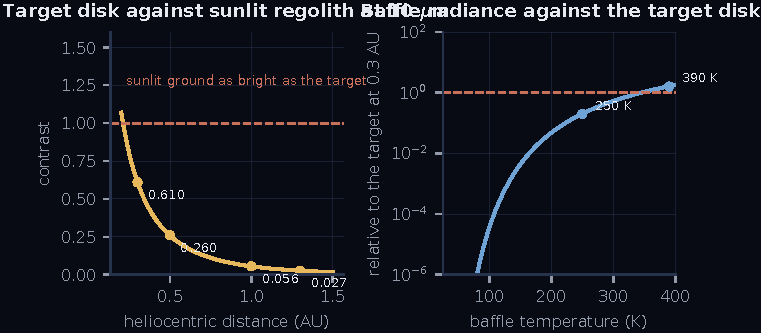
\includegraphics[width=\textwidth]{../figures/fig_mir.pdf}
\caption{Left: the contrast between a target's own thermal disk and the
sunlit lunar ground, against heliocentric distance. Below one everywhere.
Right: the radiance of a baffle at a range of temperatures against the
target's disk. The foreground is the telescope structure, not the ground.}
\label{fig:mir}
\end{figure}

\begin{table}[!htbp]
\centering
\small
\caption{Contrast between the target's thermal disk and sunlit regolith at
10 micrometres.}
\label{tab:mir-contrast}
\begin{tabularx}{\textwidth}{@{}P{1.32in}P{1.24in}Y@{}}
\toprule
\rowcolor{panel}
\textbf{Heliocentric distance} & \textbf{Contrast} & \textbf{Reading} \\
\midrule
0.3 AU & 0.61 & the target's disk is 61 per cent of the ground's \\
\rowcolor{panel}
0.5 AU & 0.26 & the ground is four times brighter \\
1.0 AU & 0.055 & the ground is eighteen times brighter \\
\rowcolor{panel}
1.3 AU & 0.027 & the ground is thirty-seven times brighter \\
\bottomrule
\end{tabularx}
\end{table}

In every heliocentric distance at which these objects are scientifically
interesting, the sunlit lunar ground is brighter than the asteroid's own
thermal emission. \tabref{tab:mir-contrast} is the first half of the case
against a lunar mid-infrared channel.

\section{The foreground is the telescope, not the ground}

The second half is more interesting, because it changes the engineering
conclusion rather than just the feasibility one.

The ground is not what the instrument looks at. The instrument looks along a
baffle or a sunshade, and the baffle has its own temperature and its own
radiance. A baffle at 390 kelvin is 1.6 times brighter than the target's
disk; a baffle at 250 kelvin is a factor of five fainter than the target and
entirely workable; a baffle at 40 kelvin is smaller by seventeen orders of
magnitude.

So the lunar mid-infrared channel is not forbidden by the background. It is
a cryogenic-optics problem: the optics must be held near 40 kelvin while
sitting on 390 kelvin regolith, with no atmosphere to reject heat into and
no radiative path other than deep space.

\begin{deeper}{What this means for the proposal}
The difference between a background problem and an engineering problem is the
difference between a channel that cannot exist and a channel that costs a
cryostat and ten kilowatts. The book states the second, because the second
is what an engineering study would have to answer. But the answer is
expensive, and Chapter 26 shows that a platform already exists that answers
it for less.
\end{deeper}

\section{The two cures, and their prices}

The cold cure is a permanently shadowed region, where the ground sits at 25
to 40 kelvin. The foreground there is lower than the target's disk by
seventeen to nineteen orders of magnitude, so the thermal problem vanishes
completely.

The price is that a permanently shadowed region receives no sunlight and
therefore has no power. The power cure is published by NASA: combining
regenerative fuel cells with a vertical solar array technology ``enables
supply and recharge of 10KW of power to permanently shadowed regions on the
Moon''. The deployable mast concept is the same idea in hardware form.

The price of the power cure is a 10 kilowatt-class power system, a cryogenic
instrument, and a night that runs for 328 hours. The instrument survival
temperatures are about 100 kelvin, and a seven kilowatt-hour battery is
needed to carry a spectrometer through the lunar night.

\begin{table}[!htbp]
\centering
\small
\caption{The mid-infrared channel: what it costs on the Moon, and what the
comparison platform already provides.}
\label{tab:mir-comparison}
\begin{tabularx}{\textwidth}{@{}P{1.24in}P{1.32in}Y@{}}
\toprule
\rowcolor{panel}
\textbf{Parameter} & \textbf{Lunar surface} & \textbf{Sun-Earth L1} \\
\midrule
Aperture & as chosen & 0.5 m, already specified \\
\rowcolor{panel}
Band & 5 to 14 micrometres & 4 to 5.2 and 6 to 10 micrometres \\
Detector temperature & about 40 K & 40 K \\
\rowcolor{panel}
Passive cooling & requires a permanently shadowed region & a space
radiator, no regolith, no dust, no night \\
Status & a concept & two funded missions \\
\bottomrule
\end{tabularx}
\end{table}

\tabref{tab:mir-comparison} is the comparison that decides the channel. The
European Space Agency's NEOMIR concept has a 50-centimetre telescope
passively cooled below 60 kelvin with detectors at 40 kelvin, a 6 to 10
micrometre band, a 30 to 70 degree solar elongation field of regard and no
atmosphere, no dust and no night. NASA's NEO Surveyor has a 50-centimetre
telescope on a halo orbit at Sun-Earth L1 with 4 to 5.2 and 6 to 10
micrometre channels. Both are the same aperture, both at 40 kelvin, and
neither has to survive regolith.

\section{The verdict}

The verdict on the thermal channel is therefore not that the Moon cannot do
it. It is that a space telescope does it better and more cheaply, and the
comparison decides it.

That is a loss, and the book records it as a loss. The proposal that follows
in Chapter 25 has no mid-infrared channel, and the optical channel is the
one it carries. This is not a retreat from the original concept; it is the
consequence of taking the arithmetic seriously, and it makes the proposal
smaller, cheaper and more defensible.

\begin{keytakeaways}
\item Sunlit regolith at 390 kelvin is brighter than the target's own
thermal disk at every heliocentric distance of interest, with contrasts
from 0.61 down to 0.027.
\item The real foreground is the baffle, which is 1.6 times the target at
390 kelvin and seventeen orders of magnitude below it at 40 kelvin, so the
channel is an engineering problem rather than an impossibility.
\item The cold cure is a permanently shadowed region, which has no power,
and the power cure is a 10 kilowatt-class system that has to survive a
328-hour night.
\item The comparison decides the channel: a 0.5-metre telescope at
Sun-Earth L1 is already specified for it, at 40 kelvin, with no regolith.
\end{keytakeaways}
